\chapter{Introduction} 

\section{Solver theory -- TODO}

\subsubsection{Euler}
Take derivative, multiply with timestep, add to initial value, repeat until end.

\subsubsection{Runge-Kutta methods}
Take derivatives at some time points, multiply with proper coefficients, add all to intial value, repeat until end.

\subsubsection{Stability}

\section{What is FP -- TODO}
Should I add a section on this to make everything understandable to all readers?


\section{Using Haskell for numerical mathematics}
Functional languages have several properties which make them suitable for the purpose of solving problems in numerical mathematics. First and foremost, Haskell, being based on $\lambda$-calculus is very close to mathematics. The useful mathematical properties here are \textit{referential transparency}, easy \textit{partial function application} and being a \textit{declarative language}. 
Referential transparency implies that a variable only has a constant value which is the same everywhere in the program. This prevents that changing a variable might have influence on another computation as a side effect and it corresponds to mathematical notation. For instance, in an imperative programming like C you could write \code{i = i + 1}, which is a mathematical impossibility and therefore not allowed in Haskell. 
Partial function application is another very useful concept. Often in numerical mathematics, you want to create or process a function. You need a function that has another function as return value. For instance, take a function which requires two arguments. After only applying a single argument, the object returned still needs the second argument in order to compute the final value. This is exactly according to the definition of a function: An object that still needs arguments before being able to return its final value.
Being a \textit{declarative language} means that you write code that specifies what you want to accomplish, not how to get there. This concept is again borrowed from mathematics. You put in a set of function definitions and Haskell will figure out how to actually compute the value you request according to those definitions. This property of declarativity also has the result that Haskell is a very terse language whilst remaining easy to understand.
Secondly, Haskell has a very strong type system. The type system has three main advantages. It becomes very easy to swap out and replace functions as long as you make sure that the types are the same. The Haskell compiler will start to assert errors immediately whenever you feed it something which does not make sense or could be ambiguous which is very useful when writing programs. By having a look at the types of a Haskell program it becomes very straightforward to see what the program does and how it works, which is very useful when attempting to understand your own or someone else's code.
Lastly, a property which is often very important for numerical mathematics: Haskell is fast. According to the \textit{Computer Language Benchmarks Game} \cite{Bench}, Haskell is almost on par with Java and Fortran but significantly faster than Python and Matlab (not shown), two languages which are often used for numerical mathematics nowadays. There is still a performance gap of around a factor 3 between Haskell and C (the reference), hence if speed is of the absolute highest concern C is still a valid option.

\section{Numerical solutions of ODEs in Haskell}
\lstset{style=haskellStyle}

As mentioned before, the types in Haskell reveal lots of information about the structure and functionality of the program. The three main types constituting the numerical solver for ordinary differential equations are listed above.

\lstinputlisting[caption=Main types for the ODE solver, label=solvertypes, firstline=18]{../haskell/SolverTypes.hs}

\subsubsection{Equation}
In essence, a differential equation is a mapping (function) from a certain state of the system to the change of this system. This is also what the type signature of \code{Equation} signifies, a mapping from an \code{ODEState} to a \code{D_ODEState}. This generic set up allows the specification of any ODE for solving. The implementation in pure Haskell of a simple ODE is given in listing \ref{lst:eq_exponential}, which corresponds to the equation $x' = -x$. However, this representation is not very elegant and a lot of the code is performing unboxing of the types. Using property that this equation is linear, it is possible to use an utility method which takes as input a matrix and returns the Haskell differential equation function belonging to that matrix. The same can be done for heterogeneous linear systems using a different utility function, which does not only takes a matrix as input but also a list of functions representing the heterogeneous part of the equation. The example code for this can be seen in appendix \ref{app:haskellsolver}.

\lstinputlisting[caption=Example equation for exponential decay, label=lst:eq_exponential, firstline=11,lastline=14]{../haskell/SolverEquations.hs}

\subsubsection{SolveMethod}
The \code{SolveMethod} performs the actual computations on what the next value of the solution should be: the integration scheme. In order to obtain this next state, the scheme needs three input values: It needs information on the timing constraints of the solution, in this case it needs the time step. Furthermore, it needs the equation itself and it requires the state of the system at $t_{n}$ in order to be able to determine the state of the system at $t_{n+1} = t_{n} + \Delta t$.

The most straightforward integration scheme is called forward Euler, given in equation \ref{eq:forward_euler}. Listing \ref{lst:forward_euler} depicts the translation of the mathematical expression \ref{eq:forward_euler} to Haskell. Even though some list operations have been inserted (\code{zipWith} and \code{map}), the structure is still recognizable. It computes the change in state, multiplies this with the time step obtained in line 6 and adds the initial state in line 4. Lastly, the integration scheme returns the new state of the equation, consisting of a list of x-values and a corresponding time value. Implementations of different solvers (eg. 4th order Runge-Kutta) can be found in appendix \ref{app:haskellsolver}.

\lstinputlisting[caption=Example code for the forward Euler integration scheme, label=lst:forward_euler, firstline=9,lastline=15]{../haskell/SolverSolvers.hs}

\begin{equation}
\label{eq:forward_euler}
\vecb{x}(t + \Delta t) \approx \vecb{x}(t) + \frac{\mathrm d \vecb{x}(t)}{\mathrm d t}\Delta t
\end{equation}

\subsubsection{Solver}
The \code{Solver} function in listing \ref{lst:solver_frame} acts as the main interface to the program. You specify a \code{SolveMethod}, the \code{TimeSettings} (containing the time step and the time at which to stop solving), the equation itself and an initial condition. The \code{Solver} will then return a list of states of the system. As is very common in functional programming, the \code{Solver} has been defined recursively. Line 4 is where the magic happens: the solution list is defined to be the initial condition, followed by the solution list with the new state (computed by the integration scheme on line 6) as initial condition. Additionally, there is a comparison in line 7 which ends the recursion whenever the time of the solution exceeds the maximum time value, set in the \code{TimeSettings}.

The solutions of a wide range of equations, both linear and non-linear, both homogeneous and heterogeneous and using the input matrix utility functions have been plot with suitable initial conditions to show their behavior in figure \ref{fig:solver_example}.

\lstinputlisting[caption=The main controlling function, label=lst:solver_frame, firstline=14,lastline=20]{../haskell/Solver.hs}

\begin{figure}[h!]
	\centering
	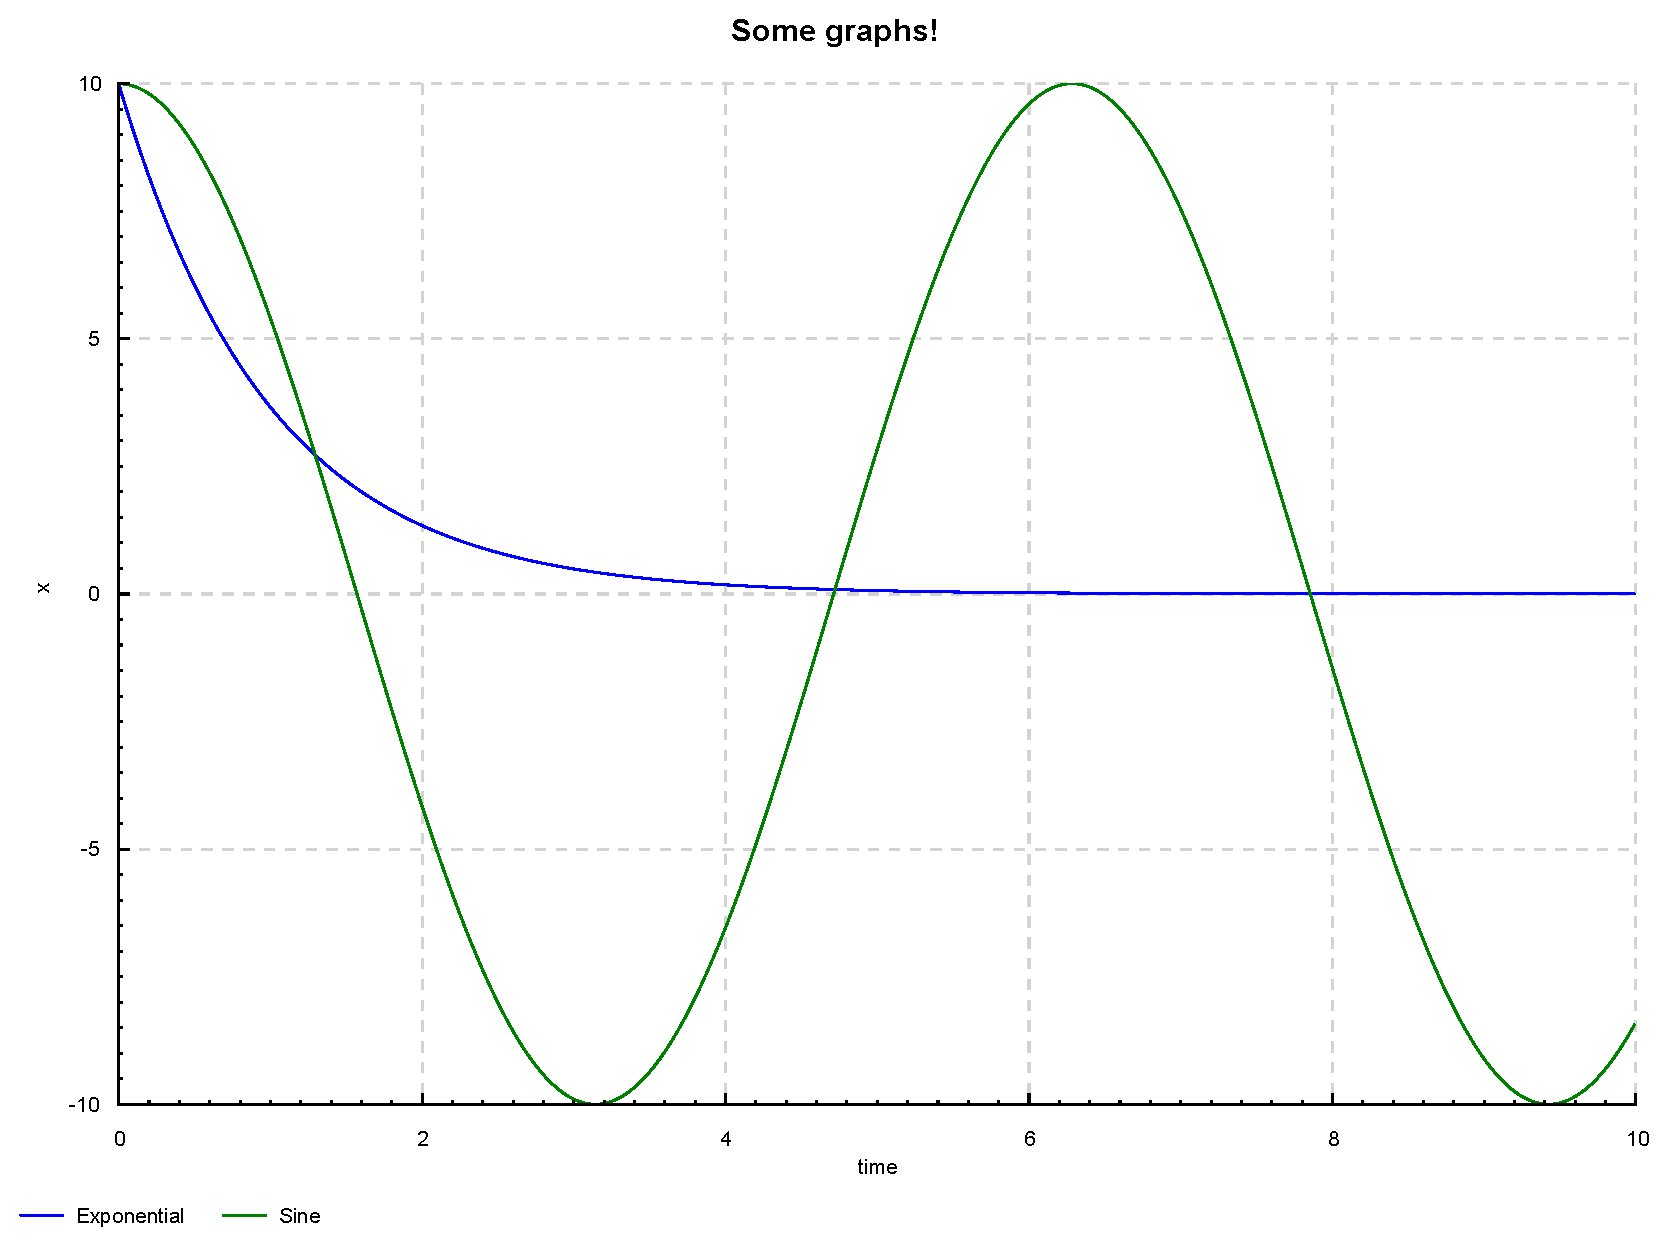
\includegraphics[width=\textwidth]{../haskell/output.pdf}
	\caption{Graphs}
	\label{fig:solver_example}
\end{figure}

\begin{align}
\text{Exponential}\sep{}			x(t)' &= -x(t)  \\
\text{Simple harmonic}\sep{}		x(t)'' &= -x(t) \\
\text{Cosine hyperbolic}\sep{}		x(t)' &= \frac{\sqrt{x(t)^{2} - a^{2}}}{a} \\
\text{Simple harmonic}\sep{}		\vecb{x}(t)' &= \begin{bmatrix} 0 & 1 \\ -1 & 0 \\ \end{bmatrix}\vecb{x}(t) \\
\text{Simple forced harmonic}\sep{}	\vecb{x}(t)' &= \begin{bmatrix} 0 & 1 \\ -1 & 0 \\ \end{bmatrix}\vecb{x}(t) + \begin{bmatrix} \sin{(t)} \\ e^{-t} \\ \end{bmatrix}
\end{align}




\section{Conversion to Mealy Machines / C$\lambda$aSH -- TODO}

Changes to:
\begin{itemize}
	\item Equation : numerical types (fixed point) - what operations would be supported in VHDL (hard to do nonlinear operators, sqrt(), sin(), cos(), tan()) - 
	\item SolutionMethod - becomes transition function of the mealy machine
	\item Solver - keeping track of the state of the solution - responsible for loading the data from the AXI-bridge to the HPS - responsible for outputting the data to the HPS for storage/processing/streaming
\end{itemize}

\iffalse
\begin{equation}
\frac{\mathrm d \vecb{x}(t)}{\mathrm d t} = f(\vecb{x}) + g(t)
\end{equation}

\begin{equation}
\frac{\mathrm d \vecb{x}(t)}{\mathrm d t} = \matr{A} \vec{x} + g(t)
\end{equation}
\fi

\section{FPGAs -- TODO}
\begin{itemize}
	\item What are FPGAs used for?
	\item Why should I care about FPGAs
	\item What is the current workflow for programming FPGAs
\end{itemize}


\section{Data transfer -- TODO}